\documentclass[12pt]{article}
\usepackage[utf8]{inputenc}
\usepackage[T1]{fontenc}
\usepackage{amsmath}
\usepackage{amsfonts}
\usepackage{amssymb}
\usepackage[version=4]{mhchem}
\usepackage{stmaryrd}
\usepackage{graphicx}
\usepackage[export]{adjustbox}
\graphicspath{ {./images/} }

\title{Problem 3. Photon Echo }

\author{}
\date{}


\begin{document}
\maketitle
The following problems will help you understand the effects of quantum optics on the different types of optical spectroscopy we all use in the lab. For all plots, you can choose the value of $\omega t$, etc for easiest graphing. Normalize your curves for easy comparison in Problem 1 and Problem 2, but not Problem 3.

\section{Linear Spectroscopy}

Linear spectroscopy is good for understanding the transition energy, but little information can be gained on lifetimes. To see this, let's look at a generalized absorption cross section:

$\sigma(\omega)=\frac{1}{6 \pi} \int d t \exp (j \omega t) \cdot\langle\mu(t) \mu(0)\rangle=\int d t \exp \left(j\left(\omega-\omega_{0}\right) t-\Gamma t-\frac{\Delta^{2} t^{2}}{2}\right)$

a. Plot the absorption cross section for $\frac{\Gamma}{\Delta}=10,0.5,0.1$ on one plot by computing the FT of the time correlation function. This represents Lorentzian, Voigt, and Gaussian lineshapes respectively. All three are commonly seen in linear spectroscopy, with the deviation from Lorentzian usually denoting inhomogeneity.

Problem 2. Pump-probe and time resolved fluorescence

Pump-probe and time resolved fluorescence measurement techniques both give the population of the excited state verse time. This allows for the population decay time to be determined, but separating dephasing is difficult.

a. Draw the evolution of the Bloch sphere for an excitation pulse with area $3 \pi / 4$ for each of the three damping cases used in Problem 1 (only $T_{1}$, mixed $T_{1}$ and $T_{2}^{*}$, only $T_{2}^{*}$ ).

b. Plot the resulting excited state decay in each of the three damping cases on one plot. The measured signal is proportional to the intensity of the response function, or

$$
I_{\text {signal }} \sim|<\mu(t) \mu(0)>|^{2}
$$

where $\langle\mu(t) \mu(0)>$ has the same form as in Problem 1. Make sure the plotted time decays match what you would predict from the Bloch diagrams. No work needed, just think.

In Problems 1 and 2, we have seen that homogenous and inhomogenous broadening is very hard to separate, although these factors determine the measured signal. If we measure the photon echo, however, we can separate these effects. The pulse train to create a photon echo is\\
shown in the following diagram:

\begin{center}
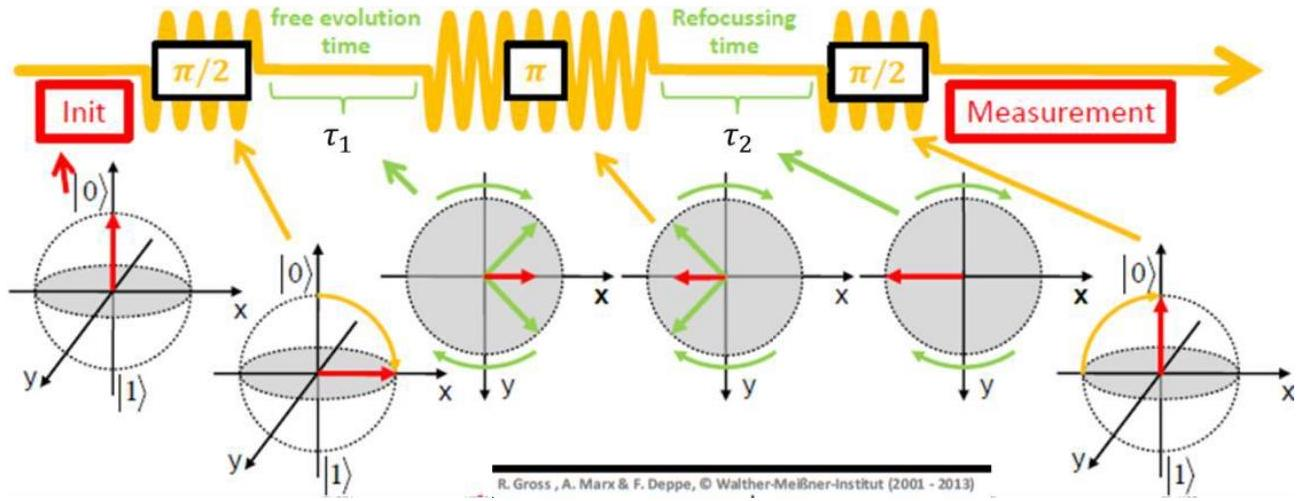
\includegraphics[max width=\textwidth]{2024_05_19_b95480aad91fe1b645d5g-2}
\end{center}

a. Plot the photon echo for the three damping constants of Problem 1 and Problem 2. The polarization for the above pulse ordered diagram can be roughly modeled as:

$$
\left|P\left(\tau_{1}, \tau_{2}\right)\right| \sim\left|R^{(3)}\right| \sim\left|\exp \left(j \omega_{0}\left(\tau_{1}-\tau_{2}\right)-\Gamma\left(\tau_{1}+\tau_{2}\right)-\frac{\Delta^{2}\left(\tau_{1}-\tau_{2}\right)^{2}}{2}\right)\right|
$$

Plot the polarization against $\tau_{2}$, taking $\tau_{1}=5, \omega_{0}=1, \Gamma=\frac{1}{2}$-and varying $\Delta=0.05,1,5$ for the three cases. Please plot all three curves on the same graph, do not normalize the heights.

You should notice the interplay between homogenous and inhomogenous broadening in the photon echo. Make sure you understand the position and shape of the photon echo based on including inhomogenous and homogenous broadening in the above Bloch diagrams. No work is needed, just think about it.

b. We can use the photon echo to separate the two broadening mechanisms. To demonstrate this, plot the photon echo against $\tau_{2}$ for several values of $\tau_{1}$. Do this for the case when the inhomogenous broadening is much larger than the homogenous ( $\Gamma=\frac{1}{2}$ and $\Delta=5$ ). Please plot all curves on the same graph, do not normalize the heights. Add a line giving the maximum value of the photon echo for all $\tau_{1}=\tau_{2}$. The result should be exponential.

The inhomogenous broadening will be rephased at a time of $2 \cdot \tau_{1}$ from the initial pulse creating a photon echo with a strength independent of the value of $\tau_{1}$. The strength of the photon echo will therefore only be determined by the extent of inhomogenous decay at 2 . $\tau_{1}$, since this cannot be reversed. Therefore, by looking at the strength of the photon echo versus $\tau_{1}$, the homogenous lifetime could be determined.

Note: The above model and response function is based on a two beam photon echo. Experimentally, three pulses are usually used and the inhomogenous and homogenous broadening are extracted a little differently from what is presented, although the use of rephasing is still the key.


\end{document}